%!TEX root = Lab-report.tex
% Добавьте ссылку на файлы с текстом работы
% Можно использовать команды:
%   \input или \include
% Пример:
%    \input{mainfiles/1-section} или \include{mainfiles/2-section}
% Команда \input позволяет включить текст файла без дополнительной обработки
% Команда \include при включении файла добавляет до него и после него команду
% перехода на новую страницу. Кроме того, она позволяет компилировать каждый файл
% в отдельности, что ускоряет сборку проекта.
% ВАЖНО: команда \include не поддерживает включение файлов, в которых уже содержится команда \include,
% т.е. не возможен рекурсивный вызов \include
\newcommand*{\Source}{
    %!TEX root = ../Lab-report.tex
\section{Постановка задачи} 
Получить аппроксимацию преобразования Фурье $F(\lambda)$ при помощи быстрого преобразования Фурье (FFT) для функций:
\begin{enumerate}
	\item $ f_1(t) = e^{-3|t|}sin^3(t) $
	\item $ f_2(t) = \frac{sin(t)-tcos(t)}{t^2} $
	\item $ f_3(t) = \frac{cos(t)}{1+|t|^3} $
	\item $ f_4(t) = e^{-5t^8}sin(t+t^3)$
\end{enumerate}

Построить графики $F(\lambda)$. Вычислить $F(\lambda)$ в явном виде для $f_1(x)$, $f_2(x)$ сравнить графики из аналитического представления и из аппроксимации через БПФ.
Проиллюстрировать эффект наложения спектра и рябь.
Проиллюстрировать устранение эффекта наложения спектра и ряби.

    %!TEX root = ../Lab-report.tex

\section{Вычисление преобразований Фурье}
$F(\lambda) = \int_{-\infty}^{+\infty} \! f(t)e^{-2 \pi i \lambda} \,dt $\\ \\
Вычислим преобразование Фурье для функции $ f_1(t) $: \\
$ sin^3(t) = \frac{1}{4}(3sin(t) - sin(3t) \Rightarrow f_1(t) = \frac{1}{4}(g(t)-h(t))$ \\
$ g(t) = 3e^{-3|t|}sin(t)$ \\
$ h(t) = 3e^{-3|t|}sin(3t) $ \\
$ f(t)sin(at) \xrightarrow{\mathscr{F}} \frac{F(\lambda - \frac{a}{2\pi}) - F(\lambda + \frac{a}{2\pi})}{2i} \Rightarrow G(\lambda) = \frac{3}{2i}(\widehat{G}(\lambda - \frac{1}{2pi}) - \widehat{G}(\lambda + \frac{1}{2pi})),$ \\ 
 $e^{-3|t|} \xrightarrow{\mathscr{F}} \widehat{G}(\lambda), $
$ \widehat{G}(\lambda) = \frac{6}{9+4 \pi^2 \lambda^2} \Rightarrow G(\lambda) = \frac{9}{i}\left[ \frac{1}{9+(1 - 2\pi \lambda)^2} - \frac{1}{9+(1 + 2\pi \lambda)^2} \right] $ \\
$ h(t) \xrightarrow{\mathscr{F}} H(\lambda) = \frac{\widehat{G}(\lambda - \frac{3}{2pi}) - \widehat{G}(\lambda + \frac{3}{2pi})}{2i} \Rightarrow H(\lambda) = \frac{3}{i}(\frac{1}{9+(3 - 2\pi \lambda)^2} - \frac{1}{9+(3 + 2\pi \lambda)^2}) $  \\
$ F_1(\lambda) = \frac{9}{4i} \left[ \frac{1}{9+(1 - 2\pi \lambda)^2} - \frac{1}{9+(1 + 2\pi \lambda)^2} - \frac{3}{9+(3 - 2\pi \lambda)^2} + \frac{3}{9+(3 + 2\pi \lambda)^2} \right] $ \\ \\
Вычислим преобразование Фурье для функции $ f_2(t) $: \\
$ f_2(t) = \frac{sin(t)-tcos(t)}{t^2} = \frac{1}{t^2}sin(t) - \frac{1}{t}cos(t) = g(t)sin(t) - h(t)cos(t)$ \\
$ g(t)sin(t) \xrightarrow{\mathscr{F}} \frac{G(\lambda - \frac{1}{2 \pi}) - G(\lambda + \frac{1}{2 \pi})}{2i}, h(t)cos(t) \xrightarrow{\mathscr{F}} \frac{H(\lambda - \frac{1}{2 \pi}) + H(\lambda + \frac{1}{2 \pi})}{2}$ \\
$ G(\lambda) = -2 \pi^2 \lambda sign(\lambda), H(\lambda) = -i \pi sign(\lambda) \Rightarrow$ \\
$ F_2(\lambda) = -\frac{\pi^2}{i} \left[ (\lambda - \frac{1}{2 \pi})sign(\lambda - \frac{1}{2 \pi}) - (\lambda + \frac{1}{2 \pi})sign(\lambda + \frac{1}{2 \pi})\right]$ + ... \\ 
... + $ \frac{i \pi}{2} \left[ sign(\lambda - \frac{1}{2 \pi}) + sign(\lambda + \frac{1}{2 \pi}) \right]$ \\
$ \Rightarrow F_2(\lambda) = i \pi^2 \lambda \left[ sign(1 - 2 \pi \lambda) + sign(1 + 2 \pi \lambda)\right]$



    %!TEX root = ../Lab-report.tex

\section{Эффект наложения спектра}
Наложение спектра возникает из-за конечной длины выборки сигнала. Если частота
Найквиста $\lambda_N$ на выбранной сетке меньше верхней границы спектральной полосы $ \lambda_{max}$, то по спектру $F_{\Delta t}(\lambda)$ дискретной функции невозможно восстановить спектр $F(\lambda)$ функции непрерывного аргумента: \\
$F(\lambda) \neq F_{\Delta t}(\lambda)H(\lambda)$ при $\lambda_N \neq \lambda_{max}$, где
$H(\lambda)$ — оконная функция. 
В этом случае в сумме периодов спектра перекрываются слагаемые
$F(\lambda - \frac{k}{\Delta x})$ и наложение окна на спектр не позволяет получить без погрешностей спектр функции непрерывного аргумента. \\

\begin{figure}[h]
\centering
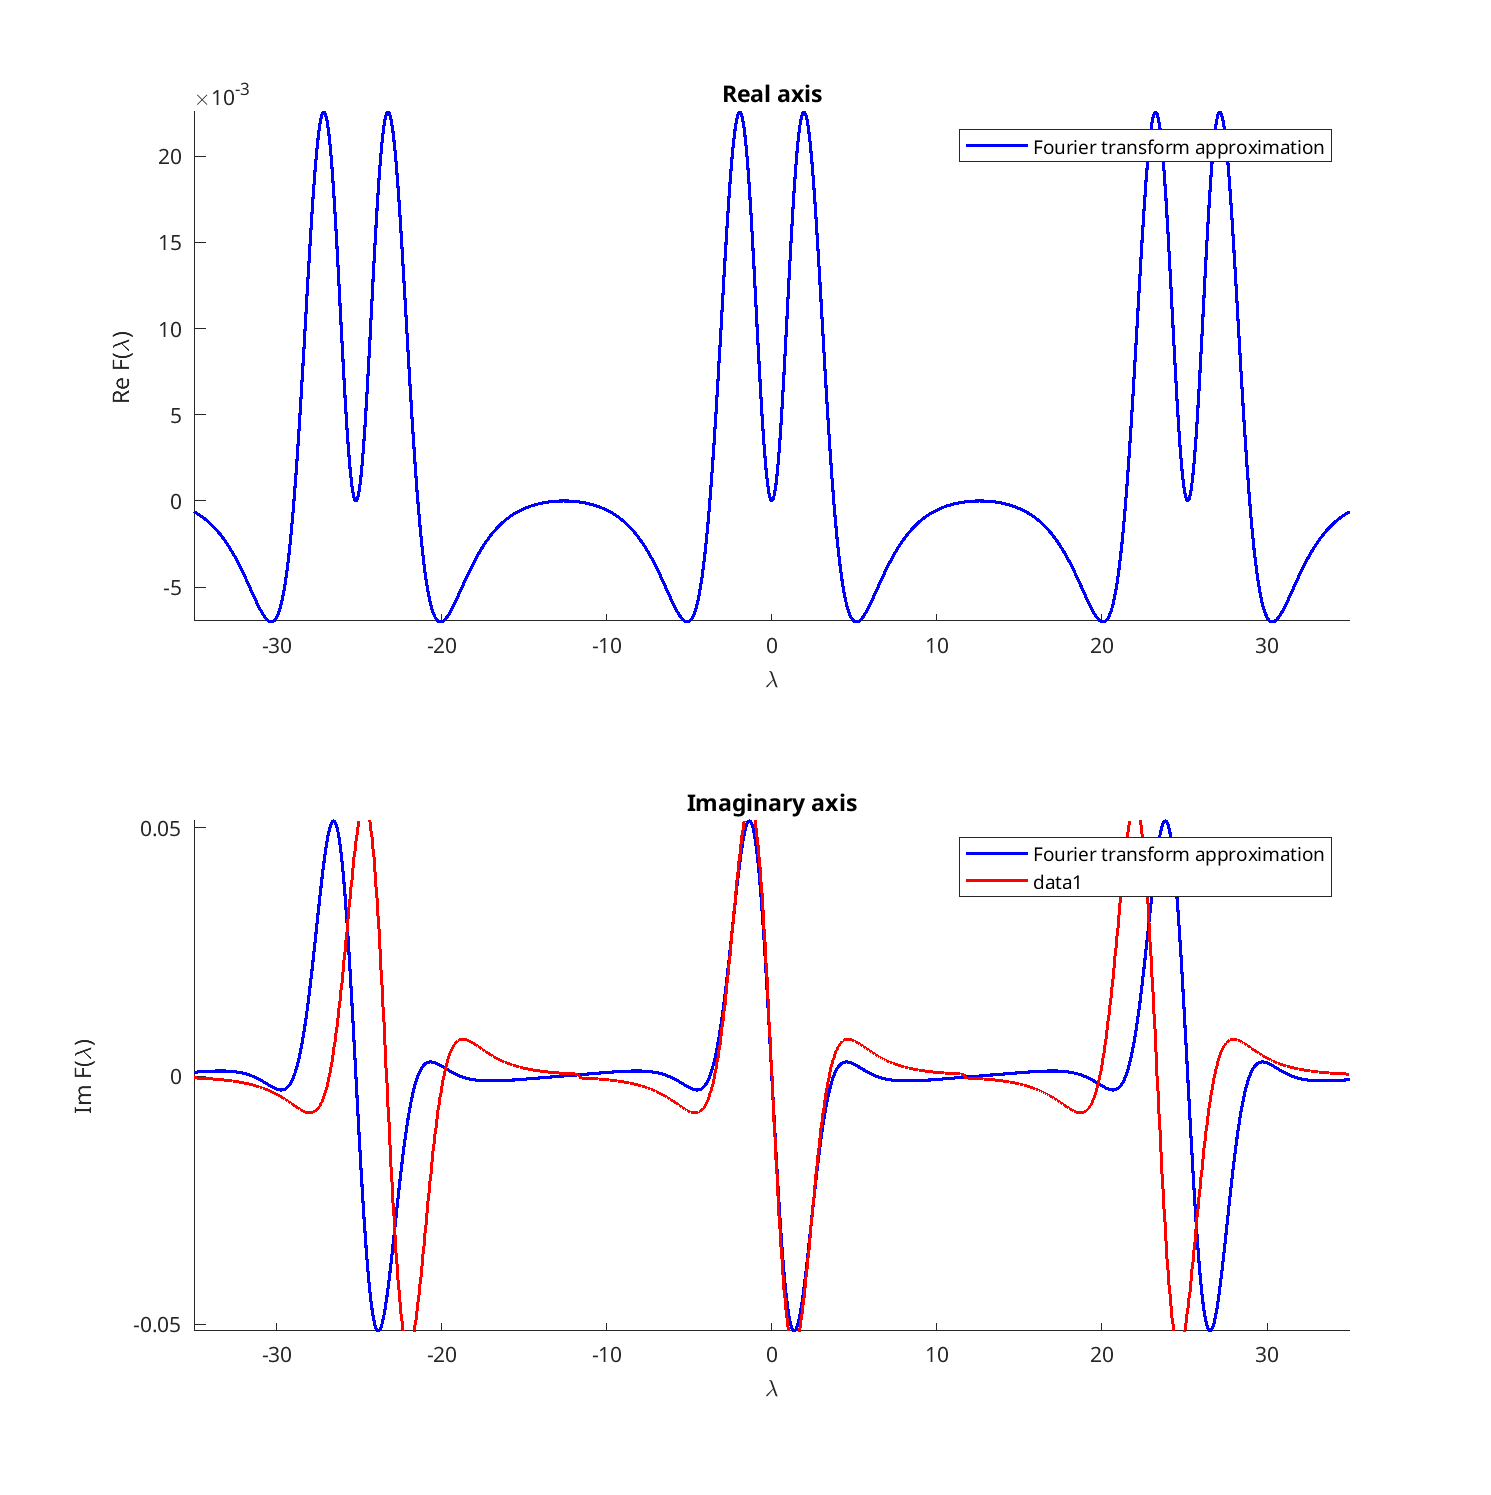
\includegraphics[width=\textwidth, height=0.5\textheight]{Aliasing-3}
\caption{$ T = 100, \Delta t = 0.25 $}
\end{figure}

\newpage

\begin{figure}[h]
\centering
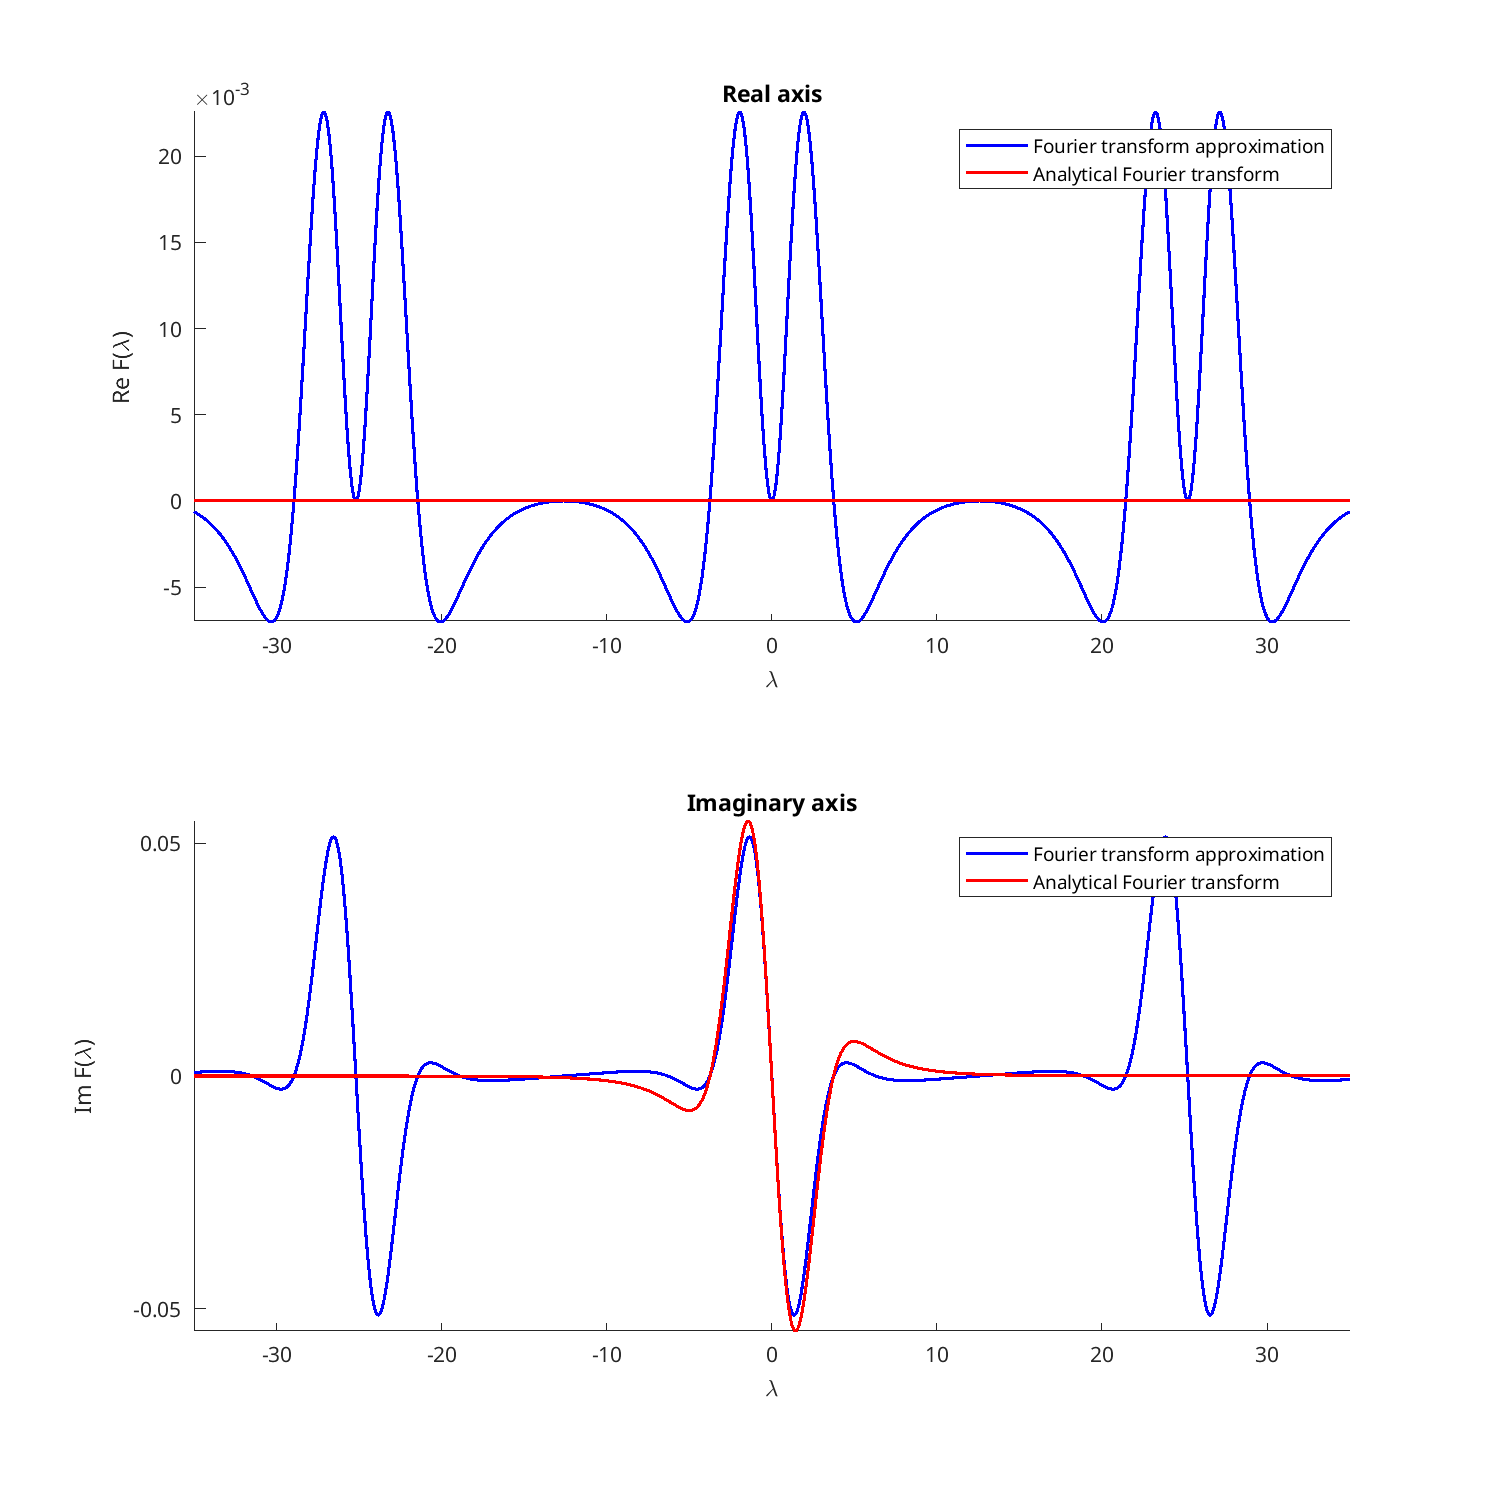
\includegraphics[width=\textwidth, height=0.35\textheight]{Aliasing}
\caption{$ T = 100, \Delta t = 0.25 $}
\end{figure}

\begin{figure}[h]
\centering
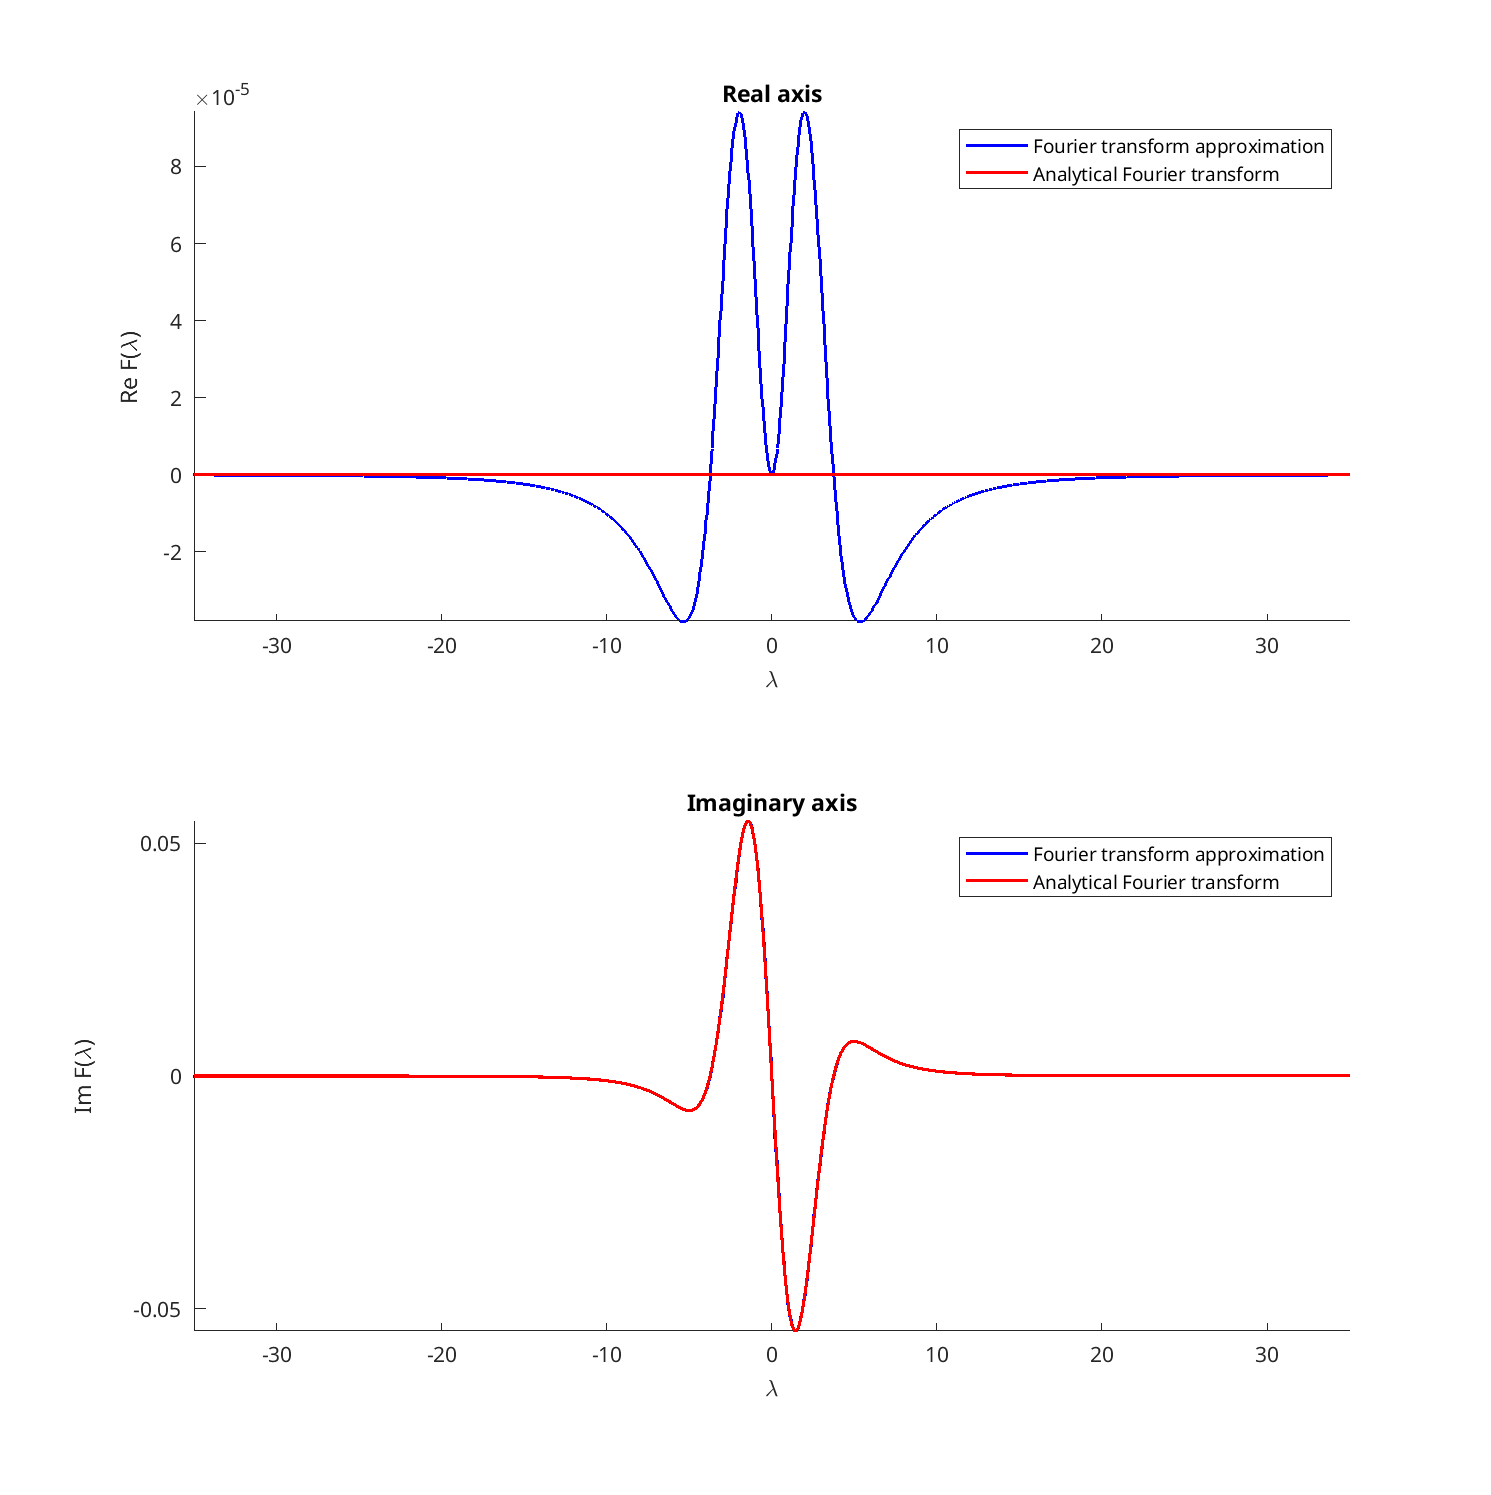
\includegraphics[width=\textwidth, height=0.35\textheight]{Aliasing-2}
\caption{$ T = 500, \Delta t = 10^{-3} $}
\end{figure}
    %!TEX root = ../Lab-report.tex

\section{Рябь}
Рябь возникает из-за усечения сигнала во временной области. Устранить этот эффект нельзя, но можно минимизировать, увеличивая временную область $[a, b] $ или частоту дискретизации сигнала. \\
\begin{figure}[h]
\centering
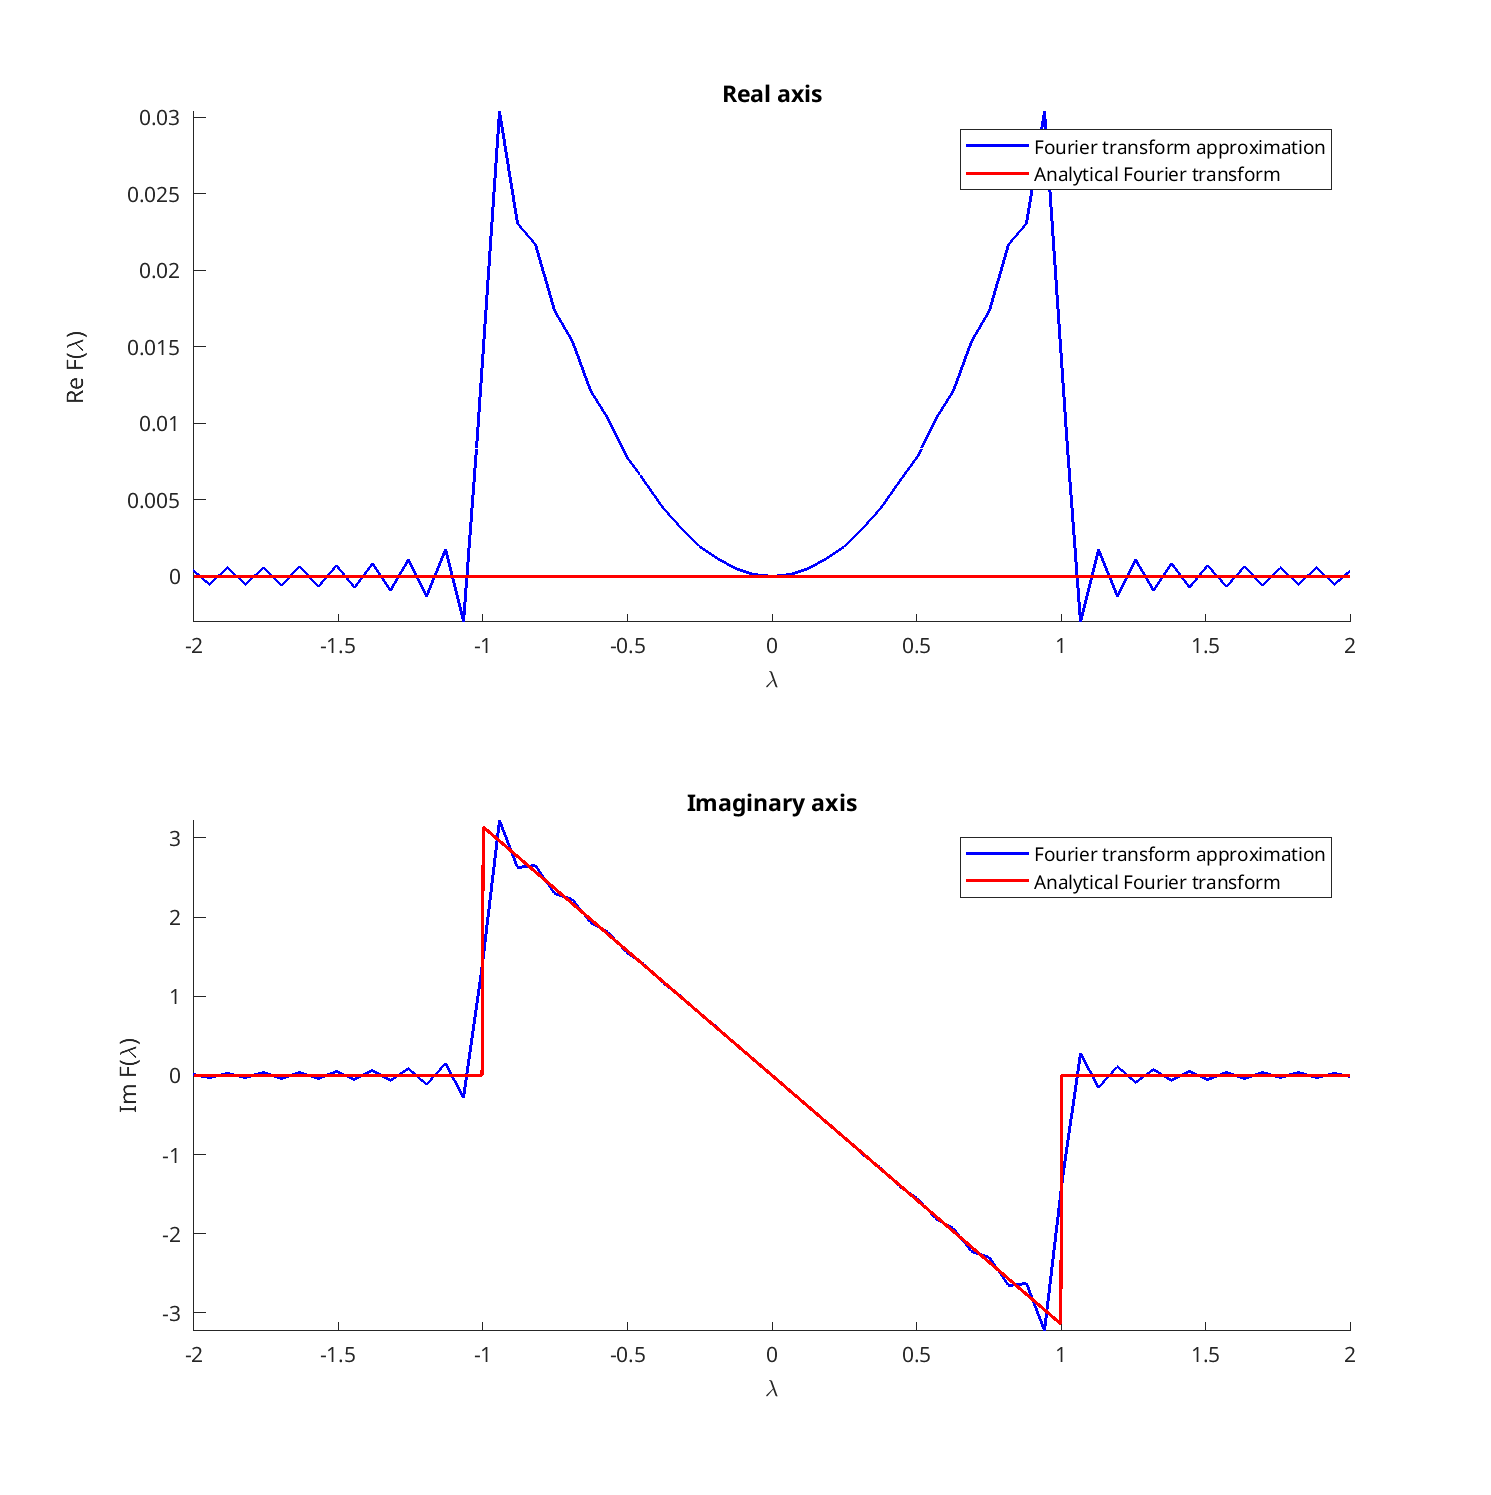
\includegraphics[width=\textwidth, height=0.7\textheight]{Gibbs}
\caption{$ T = 100, \Delta t = 0.05, t \in [-50; 50] $}
\end{figure}

\begin{figure}[h]
\centering
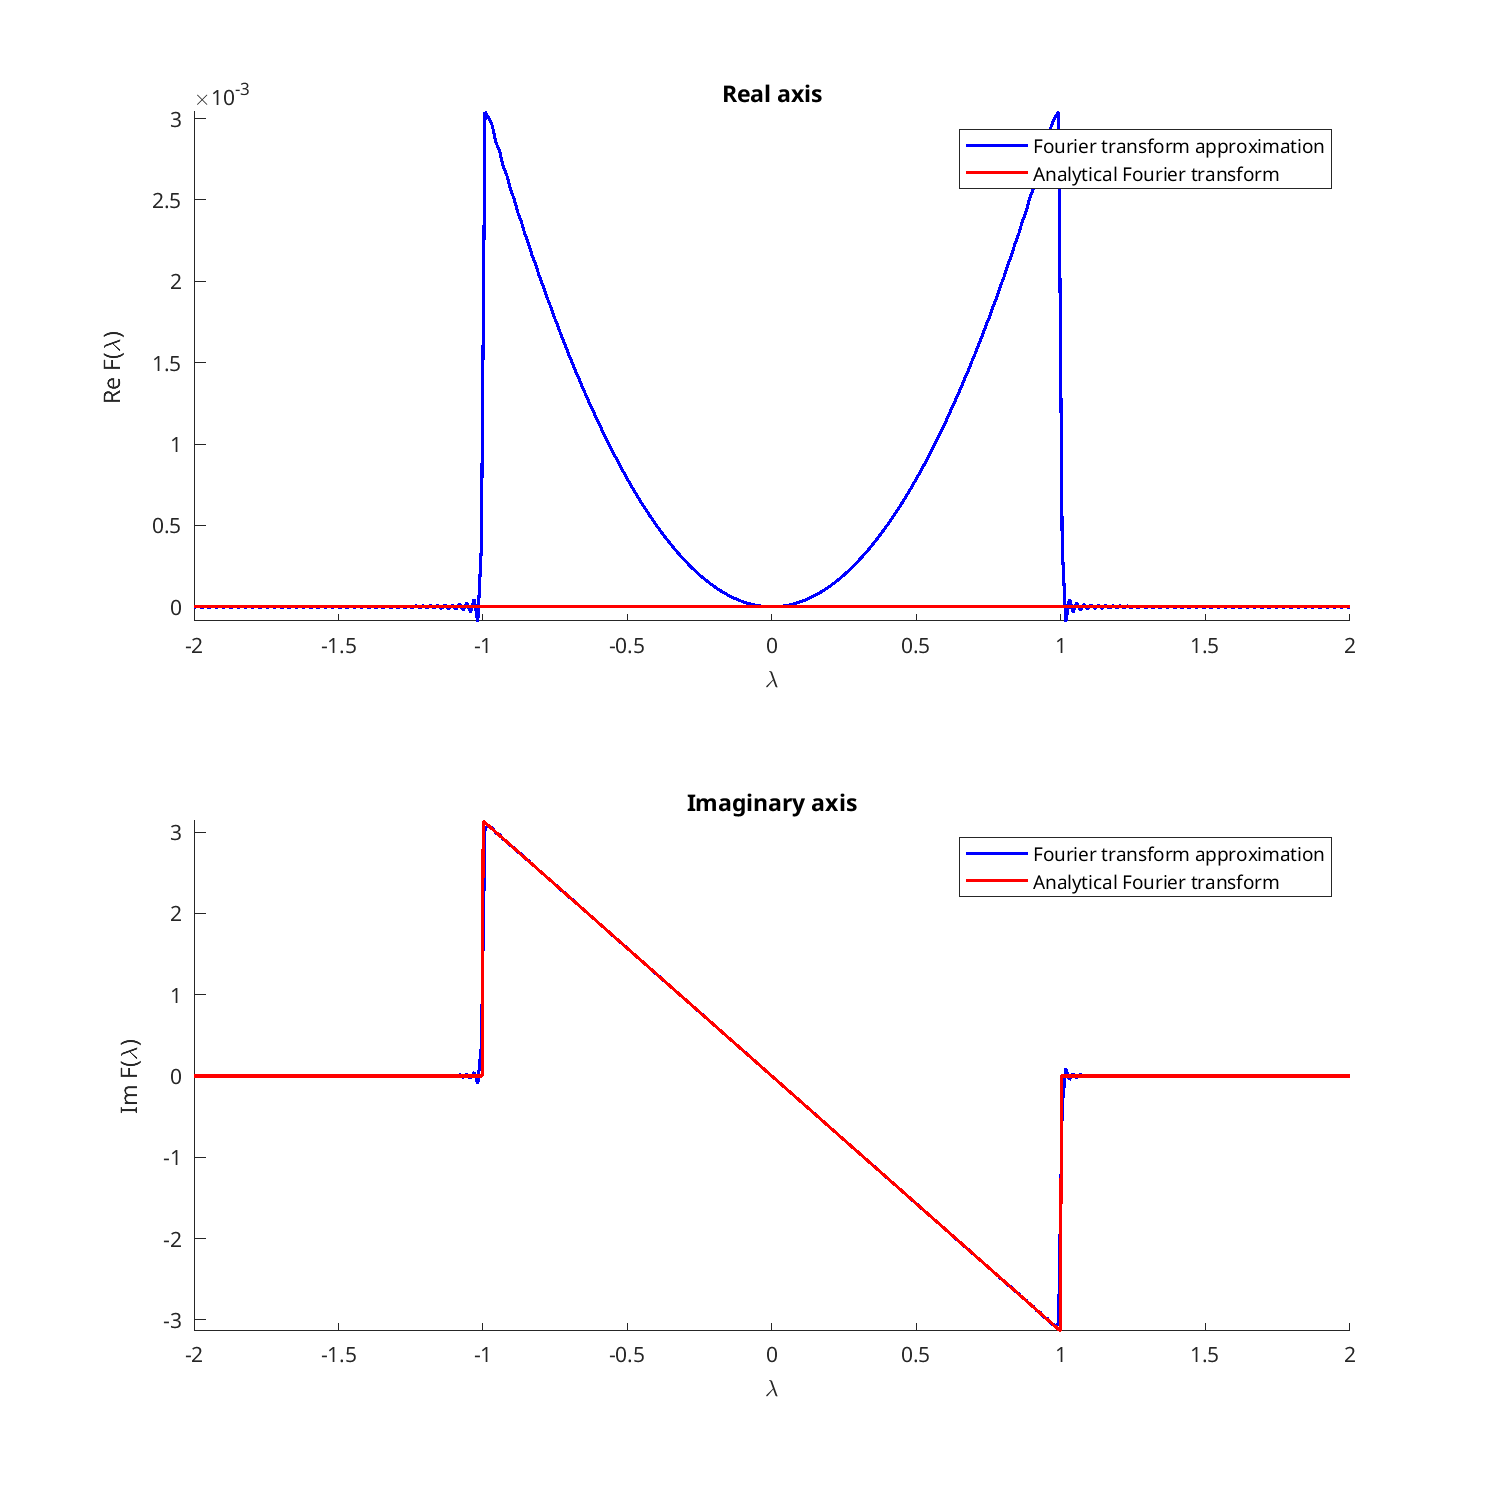
\includegraphics[width=\textwidth, height=0.7\textheight]{Gibbs-2}
\caption{$ T = 500, \Delta t = 10^{-3}, t \in [-250; 250] $}
\end{figure}
}


% Информация о годе выполнения работы
\def\Year{%
    % 2006%
    \the\year%     % Текущий год
}

% Укажите тип работы
% Например:
%     Выпускная квалификационная работа,
%     Магистерская диссертация,
%     Курсовая работа, реферат и т.п.
\def\WorkType{%
    % Выпускная квалификационная работа%
    % Магистерская диссертация%
    % Курсовая работа%
    % Реферат%
    Отчёт по практикуму
}

% Название работы
%%%%%%%%%%% ВНИМАНИЕ! %%%%%%%%%%%%%%%%
% В МГУ ОНО ДОЛЖНО В ТОЧНОСТИ
% СООТВЕТСТВОВАТЬ ВЫПИСКЕ ИЗ ПРИКАЗА
% УТОЧНИТЕ НАЗВАНИЕ В УЧЕБНОЙ ЧАСТИ
\def\Title{%
    Лабораторная работа 3%
}


% Имя автора работы
\def\Author{%
    Бачин Д.А%
}

% Информация о научном руководителе
%% Фамилия Имя Отчество%
\def\SciAdvisor{%
    Точилин Павел Александрович%
}
%% В формате: И.~О.~Фамилия%
\def\SciAdvisorShort{%
    П.~А.~Точилин%
}
%% должность научного руководителя
\def\Position{%
    % профессор%
    доцент%
    % старший преподаватель%
    % преподаватель%
    % ассистент%
    % ведущий научный сотрудник%
    % старший научный сотрудник%
    % научный сотрудник%
    % младший научный сотрудник%
}
%% учёная степень научного руководителя
\def\AcademicDegree{%
    % д.ф.-м.н.%
    % д.т.н.%
    к.ф.-м.н.%
    % к.т.н.%
    % без степени%
}

% Информация об организации, в которой выполнена работа
%% Город
\def\Place{%
    Москва%
}
%% Университет
\def\Univer{%
    Московский государственный университет имени М.~В.~Ломоносова%
}
%% Факультет
\def\Faculty{%
    Факультет вычислительной математики и кибернетики%
}
%% Кафедра    
\def\Department{%
    Кафедра системного анализа%
}     

%%%% Переключите статус документа для отладки
%%%% В режиме draft документ собирается очень быстро
%%%% и выводится полезная информация о том
%%%% какие строки вылезают за границы документа, что удобно для борьбы с ними
\def\Status{%
    % draft%
    final%
}

%%%% Включает и выключает подпись <<С текстом работы ознакомлен>>
\def\EnableSign{%
    % true%
}
